\section{Evaluation}
We first applied our approaches to several real-world dataset and compare our method with the uniform random sampling. Then we conduct several user studies on specific analysis tasks. 
\subsection{Experimental results}

Our first example uses taxi trajectories collected from 442 active taxis in the city of Porto, Portugal~\footnote{\url{http://www.geolink.pt/ecmlpkdd2015-challenge/dataset.html}}. Figure~\ref{fig:random_proposed} shows the comparison among the ground truth, uniform random sampling and the VQGTS. Both random sampling and VQGTS method take $0.01$ as the sampling rate. 
In the overview, based on the ground truth, the random sampling(shown as figure~\ref{fig:random_proposed} C) has a very poor visual quality for the boundary region. That is because 

In the overview, VQGTS(figure~\ref{fig:random_proposed} B) looks much more close to the ground truth(figure~\ref{fig:random_proposed} A) than the random method(figure~\ref{fig:random_proposed} C) especially for the boundary areas which . We further compare the details of region a and b. The figures in second row depict the detail view of the ground truth and the methods of region shown in Figure ~\ref{fig:random_proposed} a, which is the city center of Porto. Comparing with VQGTS, random sampling preserve the general trajectory framework but miss the details(As the figure~\ref{fig:random_proposed}F, G shown). For the fridge of the city where the trajectories are spare distributed, the VQGTS has clear advantage than random sampling because it well preserve the detail structure of trajectories as shown in the black region in the figure~\ref{fig:random_proposed} H and I. 

\begin{figure}[t]
	\centering
	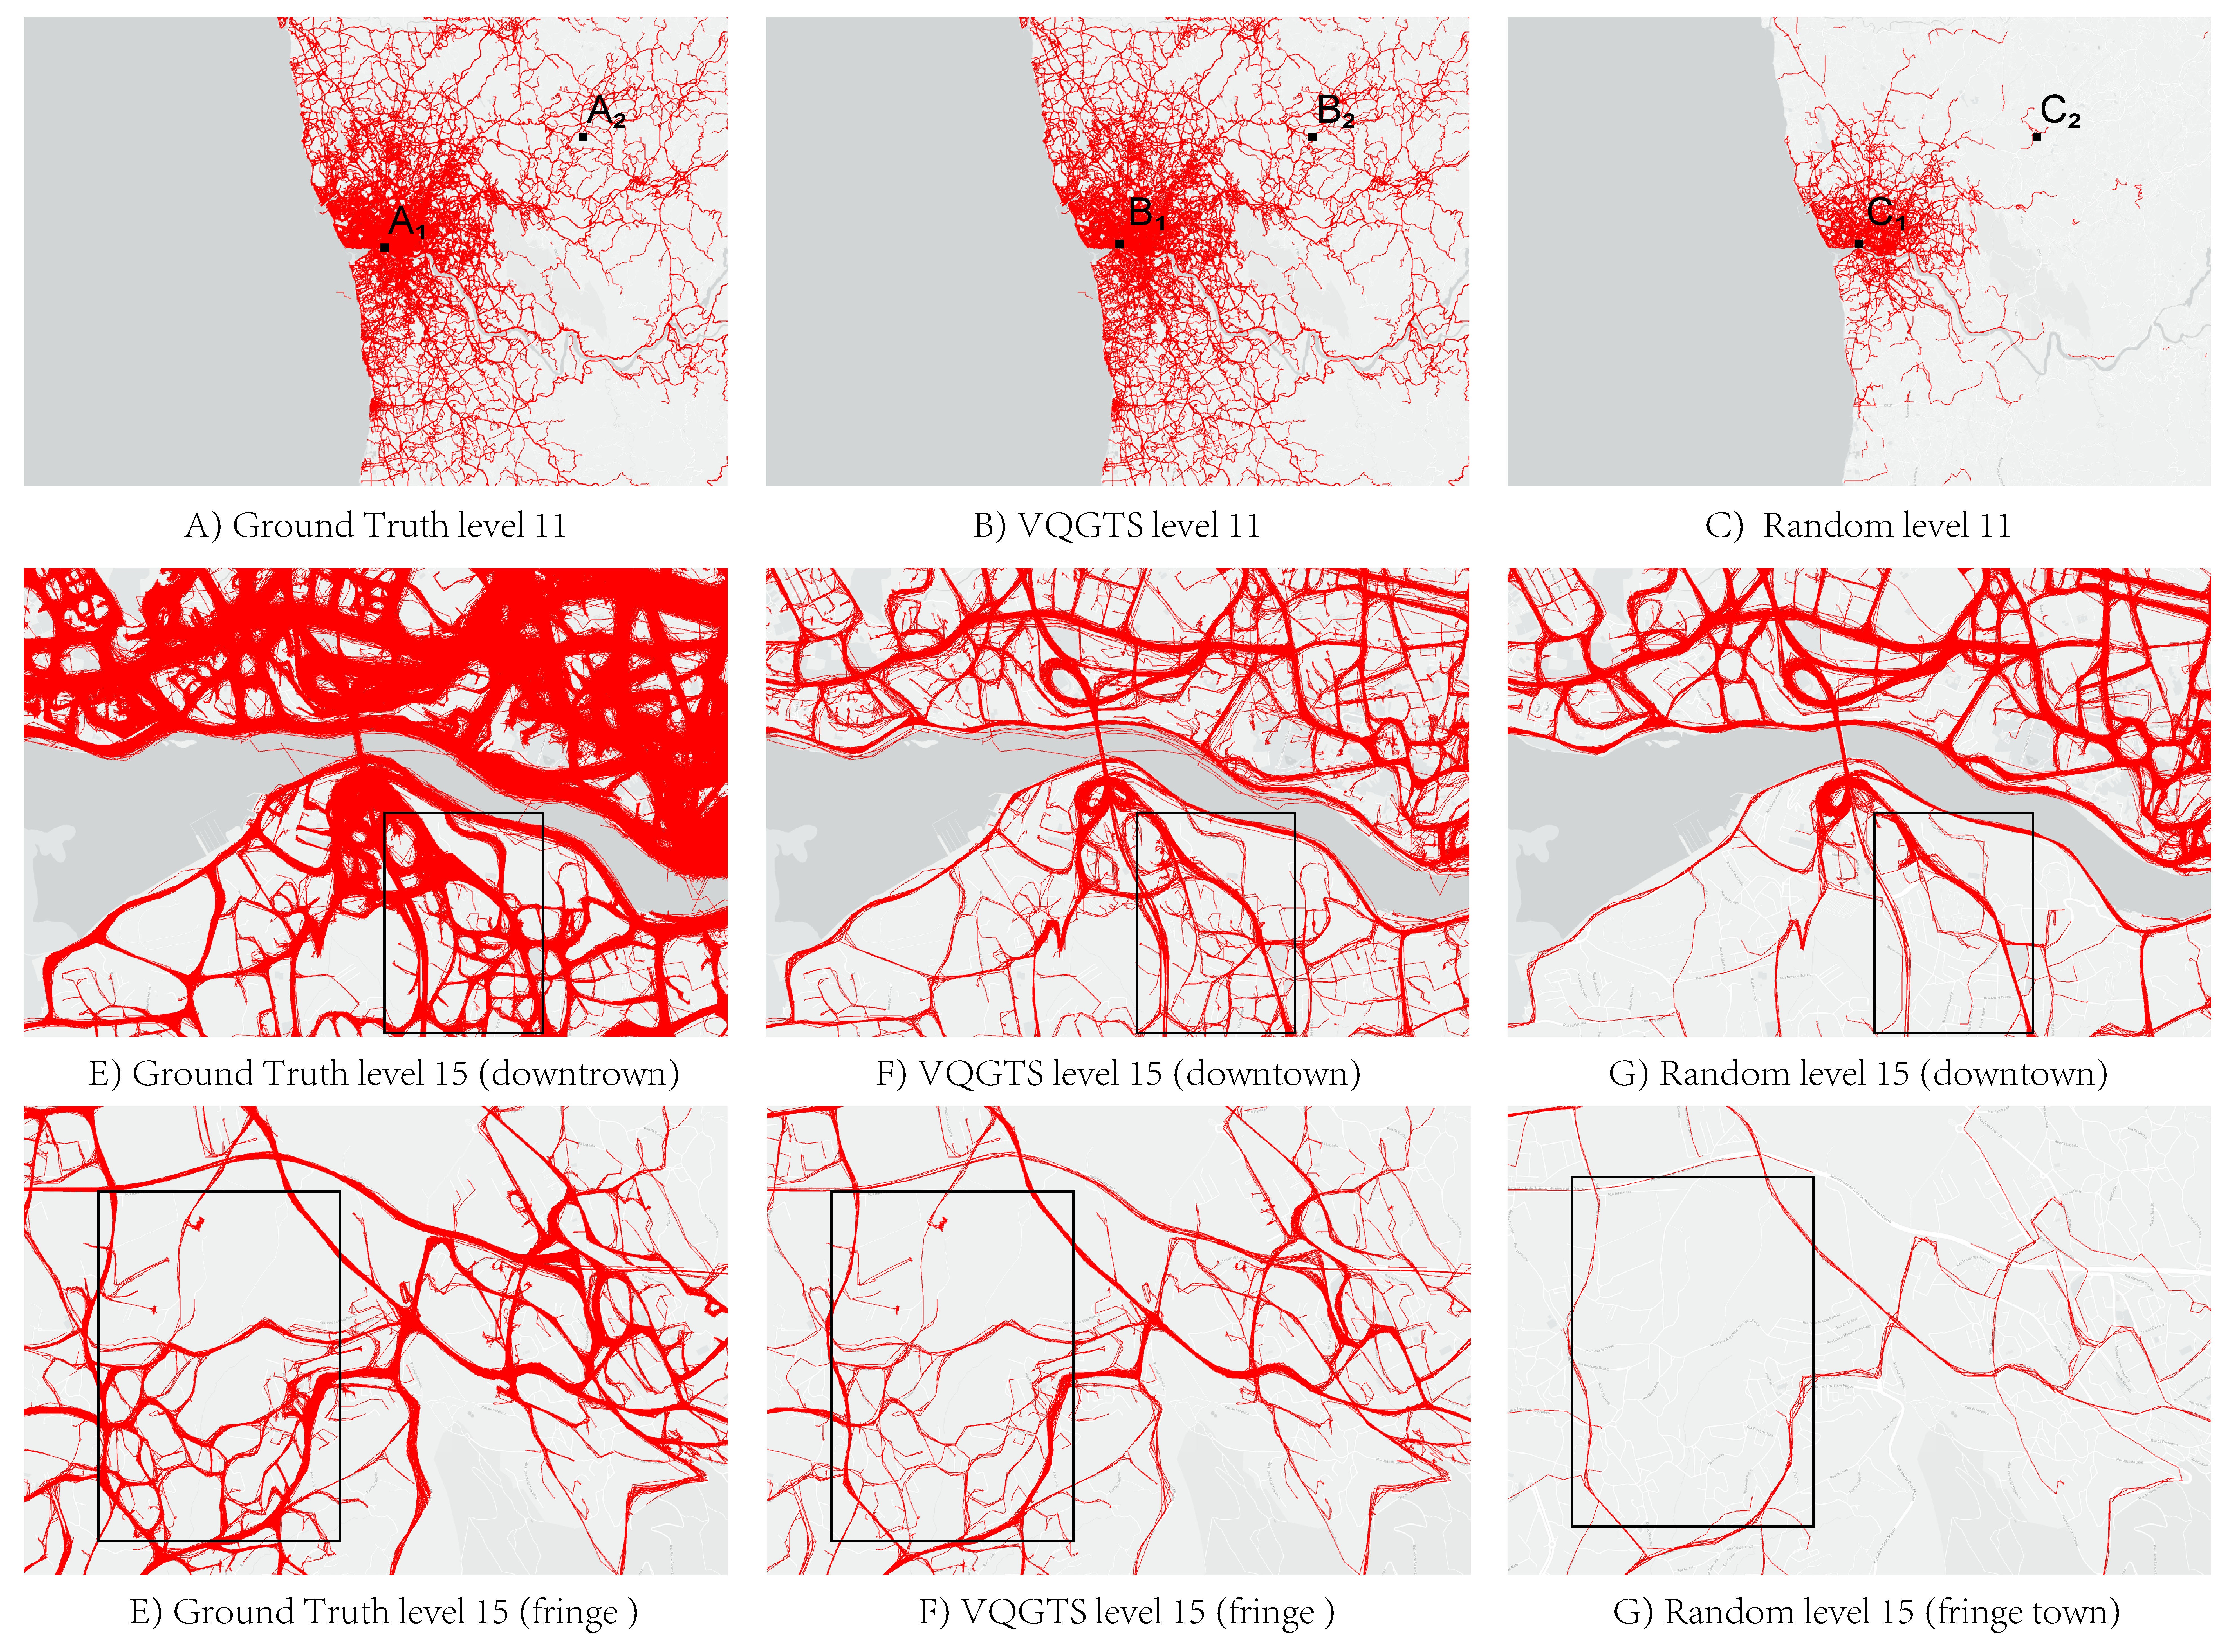
\includegraphics[width=0.48\textwidth]{pictures/experiment_study/Mehtod_resolution_study.pdf}
	\vspace{-5mm}
	\caption{Result evaluation between proposed method and uniform random sampling. The images in the three columns indicate the visualization results for full dataset, proposed method, and uniform random sampling respectively. The visualizations in the first row shows the overview. The visualizations in the second the third row indicate the detail level visualization of region 1 and region 2. }
	\vspace{-5mm}
	\label{fig:random_proposed}
\end{figure}


\subsection{User study}
\setlist{nolistsep}
\begin{itemize}[noitemsep]
    \item Visual similarity
    \item Identify outliers
\end{itemize}

\subsection{Expert overview}

